\documentclass{article}

\usepackage{amsmath}
\usepackage{enumerate}
\usepackage{graphicx}
\usepackage{caption}
\usepackage{indentfirst}

\begin{document}

\title{Application of Multilevel Models in Education Research: Effect of Reduced Class Sizes for Student Achievement}
\author{Yuwei Sun, Cheng Lu, Yifan Li}

\maketitle

\date{}

\section{Abstract}

Project STAR (Student/Teacher Achievement Ratio) was a four-year educational reform experiment conducted from 1985-1989 by the 
state of Tennessee. It was intended to investigate the effect of reduced class sizes on student achievement. In this project, 
we analyzed a subset of the data from STAR project and addressed some specific questions related to impacting factors of student 
achievement as well as a longitudinal analysis on the effect magnitude of reduced class size. Due to dependency of each data point, 
we utilized multilevel modelling techniques to conduct our analysis. Multilevel models are fitted by lmerTest package in R as 
well as the probabilistic programming language Stan, after which we compared the results and made inference about questions of interest. \\

\section{Introduction}

In STAR project, the 80 participating elementary schools throughout the state randomly assigned students entering kindergarten to 
one of three class types: small (S) with 13-17 pupils; regular (R) with 22-26 pupils or regular with a full-time teaching aide (RA) 
with 22- 26 pupils. The study lasted for four consecutive years and students information were recorded each year from kindergarten 
to third grade. Participating schools represent different geographic regions and different communities (i.e. rural, urban, suburban, 
inner city). Teachers have various backgrounds with respect to levels of education degree/experience, race etc. Students also came 
from various demographic and socioeconomic backgrounds.\\

The STAR database is extremely huge and there exist many opportunities for different analyses using all or different portions of the data. 
We have to select variables among 14 independent variables to fit model efficiently and to determine which variable should be the 
random effect. In our project we used student level as well as school level data to study the effects of a reduced pupil-teacher 
ratio on students’ read and math test scores.\\

\section{Research Questions}

Our major interest includes two aspects: how students achievements are affected by reduced class size and how the effect varies 
among other factors (socioeconomic status etc.); what other factors are associated with students’ achievements. \\

To quantify students’ achievements, we choose a subset of the dataset where the students have four-year records and stay in the 
same class type for four consecutive years  in order to simplify question and save simulation time. Our goal is to find the 
relation between mean of math scores for four years and the class type. That is, does the class type affect the students’ 
performance in math exam?\\

\section{Data}

We obtained the data from the “mlmRev” R package, which contains data and examples from a multilevel modelling software review 
as well as other well-known data sets from the multilevel modelling literature.\\

The dependent variables are math score and read score. The independent variables include student variable such as sex, race, 
socioeconomic status, teacher variable such as race, education level, race, school type and class type. The raw data contains 26,796 
observations, with 80 schools and 11598 students in total. However, several variables have a tiny portion of missing values ($< 10\%$), 
in this scenario we can assume the data is missing at random, thus we removed observations that contain missing value. 
As a consequence, we have a total of $26,796 - 3981 = 22815$ data points. The first few lines from the data frame are shown in Table 
\ref{table:data}.\\

\begin{table}[h]
    \centering
    \caption{Head of Data Frame ‘star’}
    \label{table:data}
    \begin{tabular}{|l|l|l|l|l|l|l|l|l|l|}
    \hline
    id     & sch & gr & cltype & hdeg      & clad & exp & trace & read & ... \\ \hline
    100017 & 28  & K  & small  & BS/BA     & 1    & 3   & B     & 476  &     \\ \hline
    100028 & 52  & K  & reg    & MS/MA/MEd & 1    & 12  & W     & 410  &     \\ \hline
    100045 & 41  & 1  & small  & BS/BA     & 1    & 20  & W     & 507  &     \\ \hline
    100045 & 41  & 2  & small  & MS/MA/MEd & APPR & 15  & B     & 575  &     \\ \hline
    100045 & 41  & 3  & small  & BS/BA     & 1    & 5   & W     & 610  &     \\ \hline
    ...    &     &    &        &           &      &     &       &      &     \\ \hline
    \end{tabular}
\end{table}

Here is a detailed explanation of all the variables:

\begin{enumerate}[1]

    \item \textbf{Outcome variables}:
        \begin{itemize}
            \item \textbf{read}: the student’s total reading scaled score
            \item \textbf{math}: the student’s total math scaled score 
        \end{itemize}

	\item \textbf{Student variables}:
        \begin{itemize}
            \item \textbf{id}: a factor - student id number 
            \item \textbf{ses}: socioeconomic status - a factor with levels F and N representing eligible for free lunches or not eligible 
            \item \textbf{sx}: student’s sex - a factor with levels (M, F) 
            \item \textbf{eth}: student’s ethnicity - a factor with the same levels as trace 
            \item \textbf{birthq}: student’s birth quarter - an ordered factor with levels $(1977:1 < \dots < 1982:2)$
            \item \textbf{birthy}: student’s birth year - an ordered factor with levels $(1977 < \dots < 1982)$
            \item \textbf{yrs}: number of years of schooling for the student - a numeric version of the grade gr with Kindergarten 
            represented as 0
        \end{itemize}

    \item \textbf{School variable}:
        \begin{itemize}
            \item \textbf{sch}: a factor - school id number gr grade - an ordered factor with levels $(K < 1 < 2 < 3)$
            \item \textbf{schtype}: school type - a factor with levels (inner, suburb, rural and urban)
        \end{itemize}

    \item \textbf{Class variable}:
        \begin{itemize}
            \item \textbf{cltype}: class type - a factor with levels small, reg and reg+A. The last level indicates a regular class 
            size with a teachers aide.
        \end{itemize}

    \item \textbf{Teacher variable}:
        \begin{itemize}
            \item \textbf{tch}: a factor - teacher id number
            \item \textbf{hdeg}: highest degree obtained by the teacher - an ordered factor with levels $(ASSOC < BS/BA < MS/MA/MEd 
            < MA+ < Ed.S < Ed.D/Ph.D)$
            \item \textbf{clad}: areer ladder position of the teacher - a factor with levels (NOT, APPR, PROB, PEND, 1, 2, 3)
            \item \textbf{exp}: a numeric vector - the total number of years of experience of the teacher 
            \item \textbf{trace}: teacher’s race - a factor with levels (W, B, A, H, I, O) representing (white, black, Asian, 
            Hispanic, Indian (Native American), other)
        \end{itemize}

\end{enumerate}

Summary tables for numerical variables and some important categorical variables are listed below.

\begin{table}[h]
    \centering
    \caption{summary table for numerical variables}
    \label{table:numerical variables}
    \begin{tabular}{|l|l|l|l|l|}
    \hline
    Numeric & exp   & read  & math  & yrs   \\ \hline
    Min     & 0.00  & 315.0 & 320.0 & 0.000 \\ \hline
    1st Qu  & 6.00  & 470.0 & 506.0 & 1.000 \\ \hline
    Median  & 11.00 & 553.0 & 558.0 & 1.000 \\ \hline
    Mean    & 12.13 & 541.5 & 555.3 & 1.521 \\ \hline
    3rd Qu  & 17.00 & 604.0 & 603.0 & 3.000 \\ \hline
    Max     & 42.00 & 775.0 & 774.0 & 3.000 \\ \hline
    \end{tabular}
\end{table}

\begin{table}[h]
    \centering
    \caption{summary table for some categorical variables}
    \label{table:categorical variables}
    \begin{tabular}{|l|l|l|l|l|l|}
    \hline
    sch          & cltype      & schtype      & eth      & ses      & sx       \\ \hline
    55: 744      & small: 6899 & inner: 4791  & W: 15150 & F: 11120 & M: 11763 \\ \hline
    22: 492      & reg: 7786   & suburb: 547  & B: 7539  & N:11695  & F: 11052 \\ \hline
    63: 480      & reg+A: 8130 & rural: 10759 & A: 59    &          &          \\ \hline
    9: 461       &             & urban: 1791  & H: 26    &          &          \\ \hline
    27: 453      &             &              & I: 8     &          &          \\ \hline
    7: 445       &             &              & O: 33    &          &          \\ \hline
    Other: 19740 &             &              &          &          &          \\ \hline
    \end{tabular}
\end{table}

\section{Data Preparation and Visualization}

The whole data is complicated. The total consecutive years students were followed vary from 1 to 4 years. 
Some students change class type even change school during different grade, with different teachers from various backgrounds. 
Thus, the variance source can be complicated and it’s hard to consider all the potential interactions. In addition, 
we have student level and school level as random effects, where student is nested within each school. \\

In order to reduce the magnitude of statistical computations, for this part we took a subset of observations where students 
stayed in the same class type and in the same school for four consecutive years (K-1-2-3), after which data were aggregated 
to the level of individual student means of 4 years’ test score. Due to aggregation, we only kept independent variables which 
are constant for each student among the four years: ses, sx, eth, birthq, birthy, cltype, sch, schtype. This subset contains 
1124 observations, with 69 schools in total.\\

\begin{minipage}{\linewidth}
    \makebox[\linewidth]{
      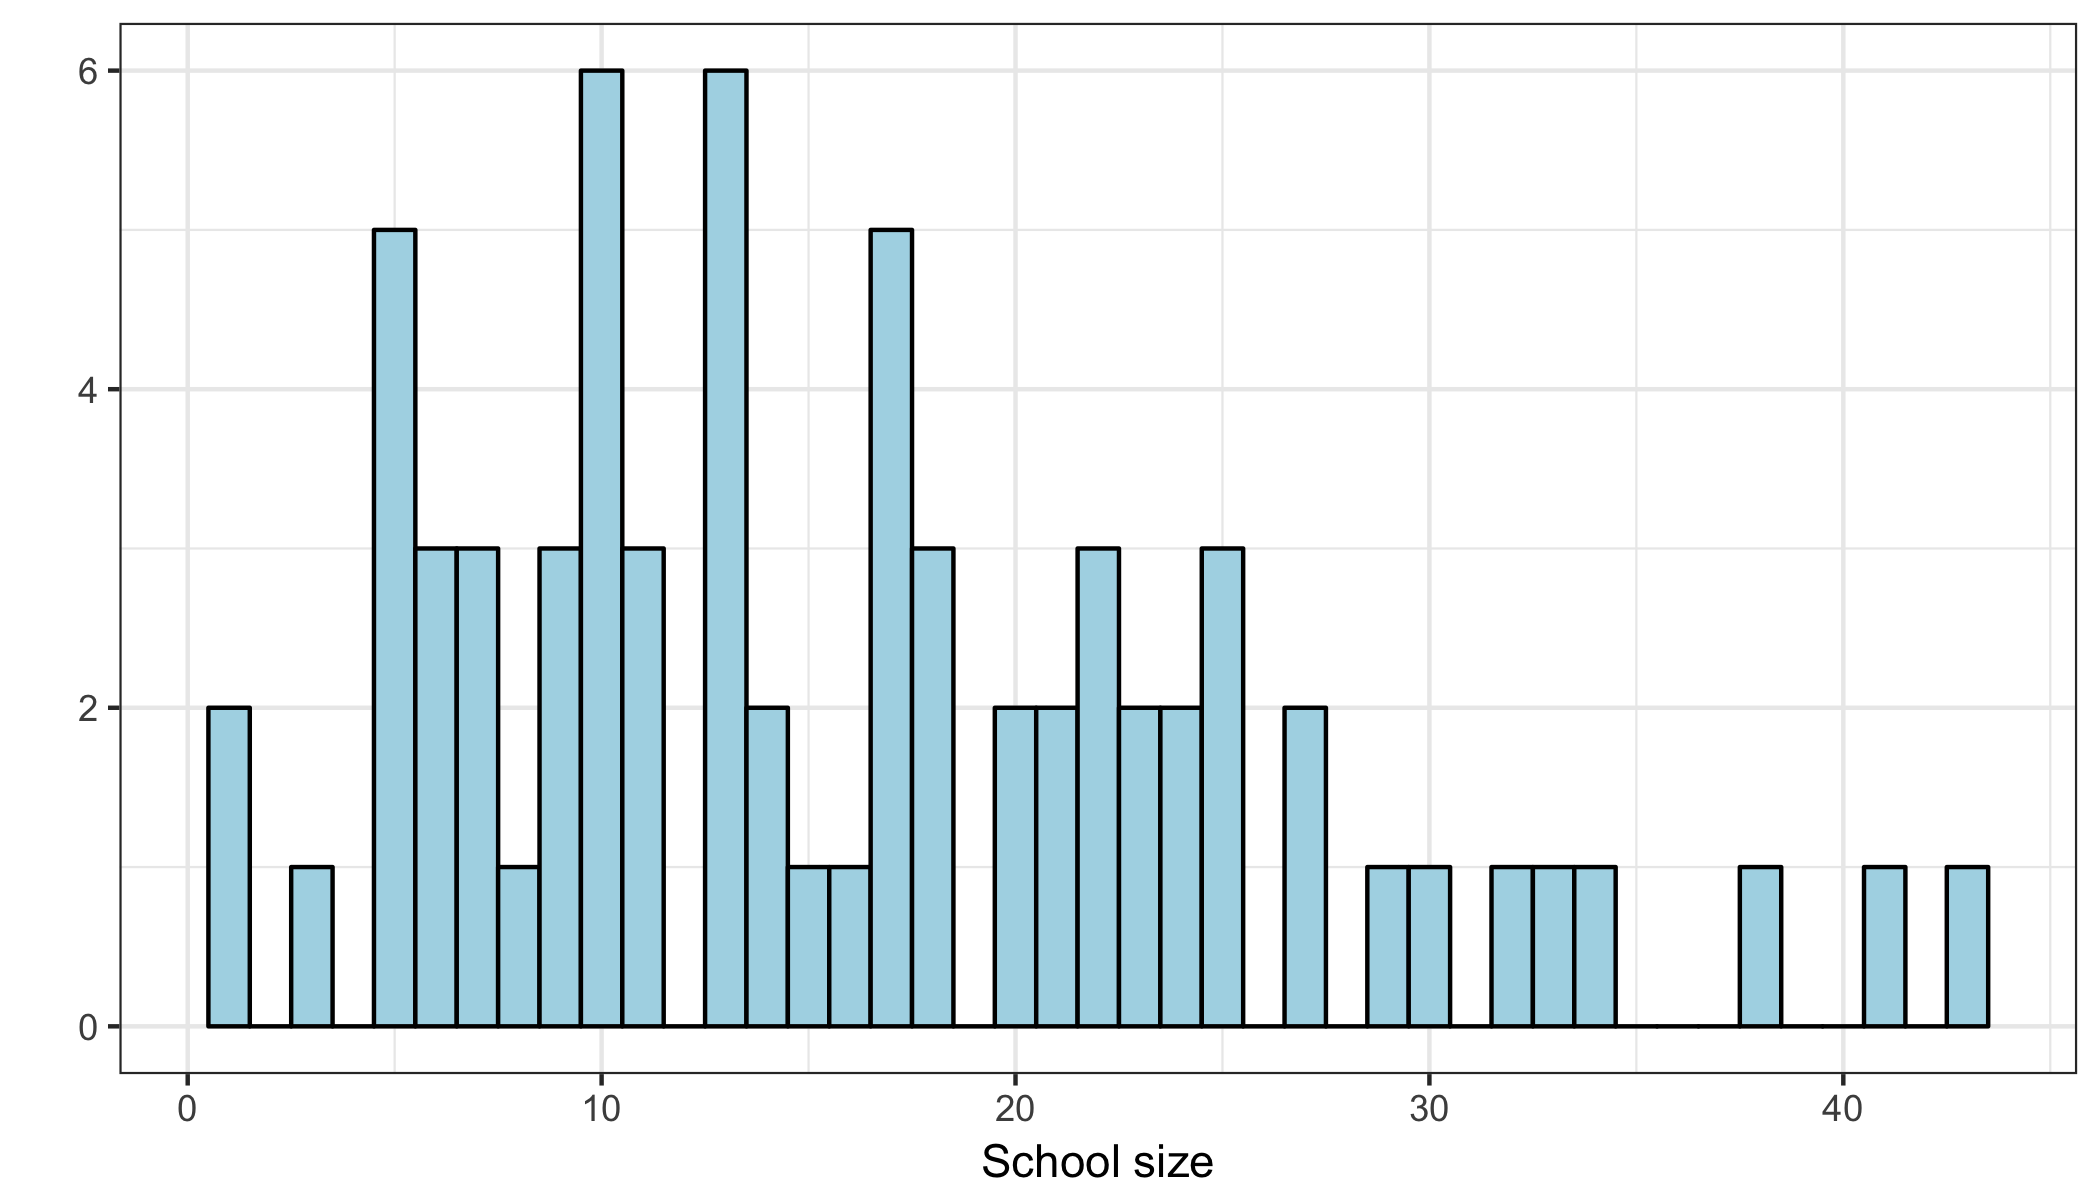
\includegraphics[scale=0.15]{../plot/school.png}
      }
    \captionof{figure}{School Size}\label{fig:school}
\end{minipage}\\

From Fiture \ref{fig:school}, the number of data in different schools is unbalanced. Because of this, 
variable 'sch' is taken as a random effect.\\

\begin{minipage}{\linewidth}
    \makebox[\linewidth]{
      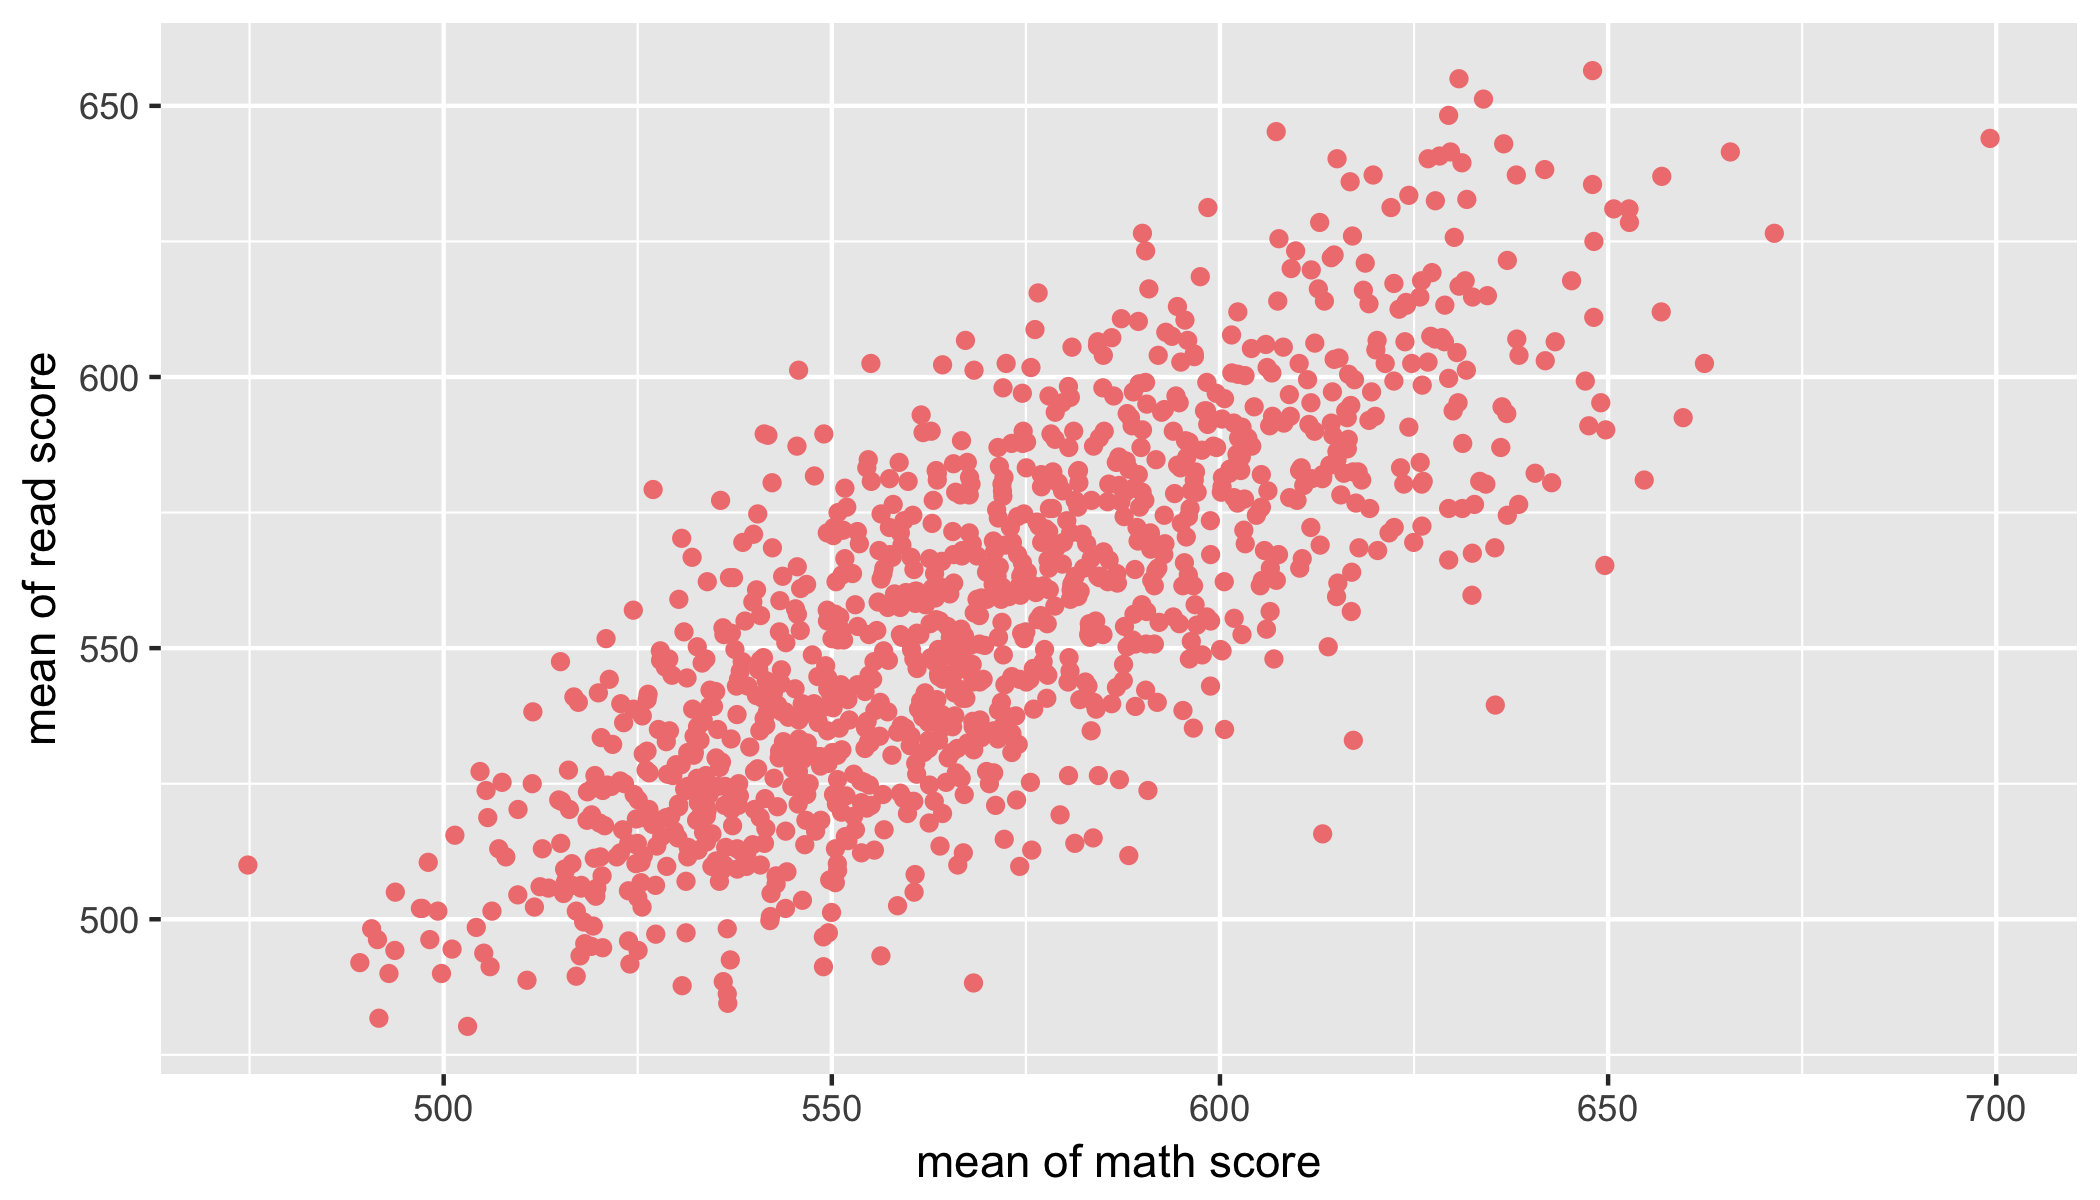
\includegraphics[scale=0.15]{../plot/mathread.png}
      }
    \captionof{figure}{math vs read}\label{fig:mathread}
\end{minipage}\\

From Fiture \ref{fig:mathread}, we can see that there is a obvious linear relation between the mean of math score and the mean of read score, 
which means we can choose either of the two to be our dependent variable. We just choose the mean of math score to be our response.\\

\begin{minipage}{\linewidth}
    \makebox[\linewidth]{
      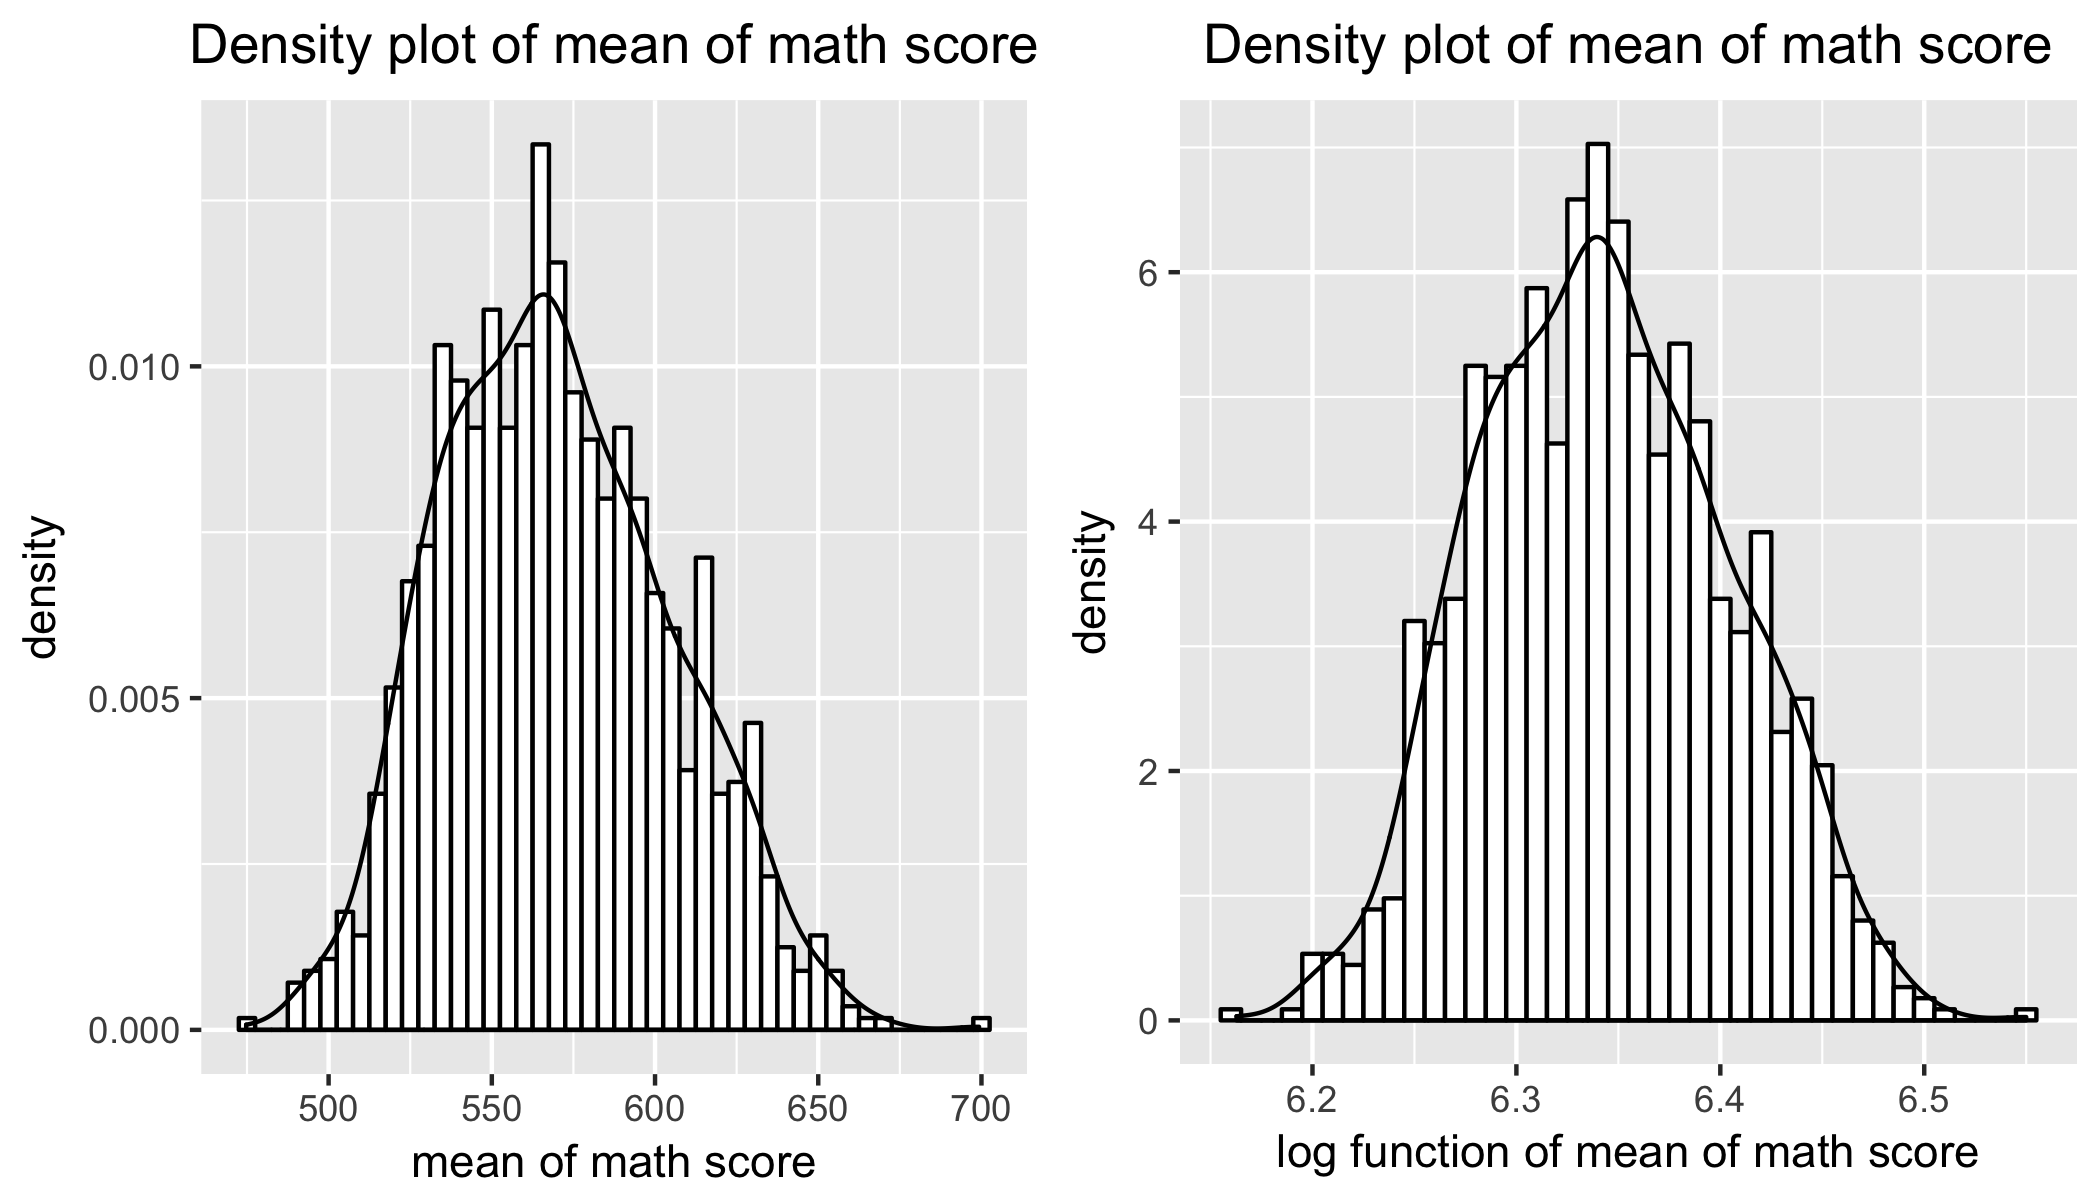
\includegraphics[scale=0.15]{../plot/math.png}
      }
    \captionof{figure}{Distribution of math}\label{fig:math}
\end{minipage}\\

From Fiture \ref{fig:math}, the distribution of math score is closed to normal distribution. And after $\log$ transformation, 
the assumption of normal distribution does not improve much. So math is taken as dependent variable without transformation.\\

Next, we draw the plot to obtain the relation between the mean of math score and the other variables.\\

\begin{minipage}{\linewidth}
    \makebox[\linewidth]{
      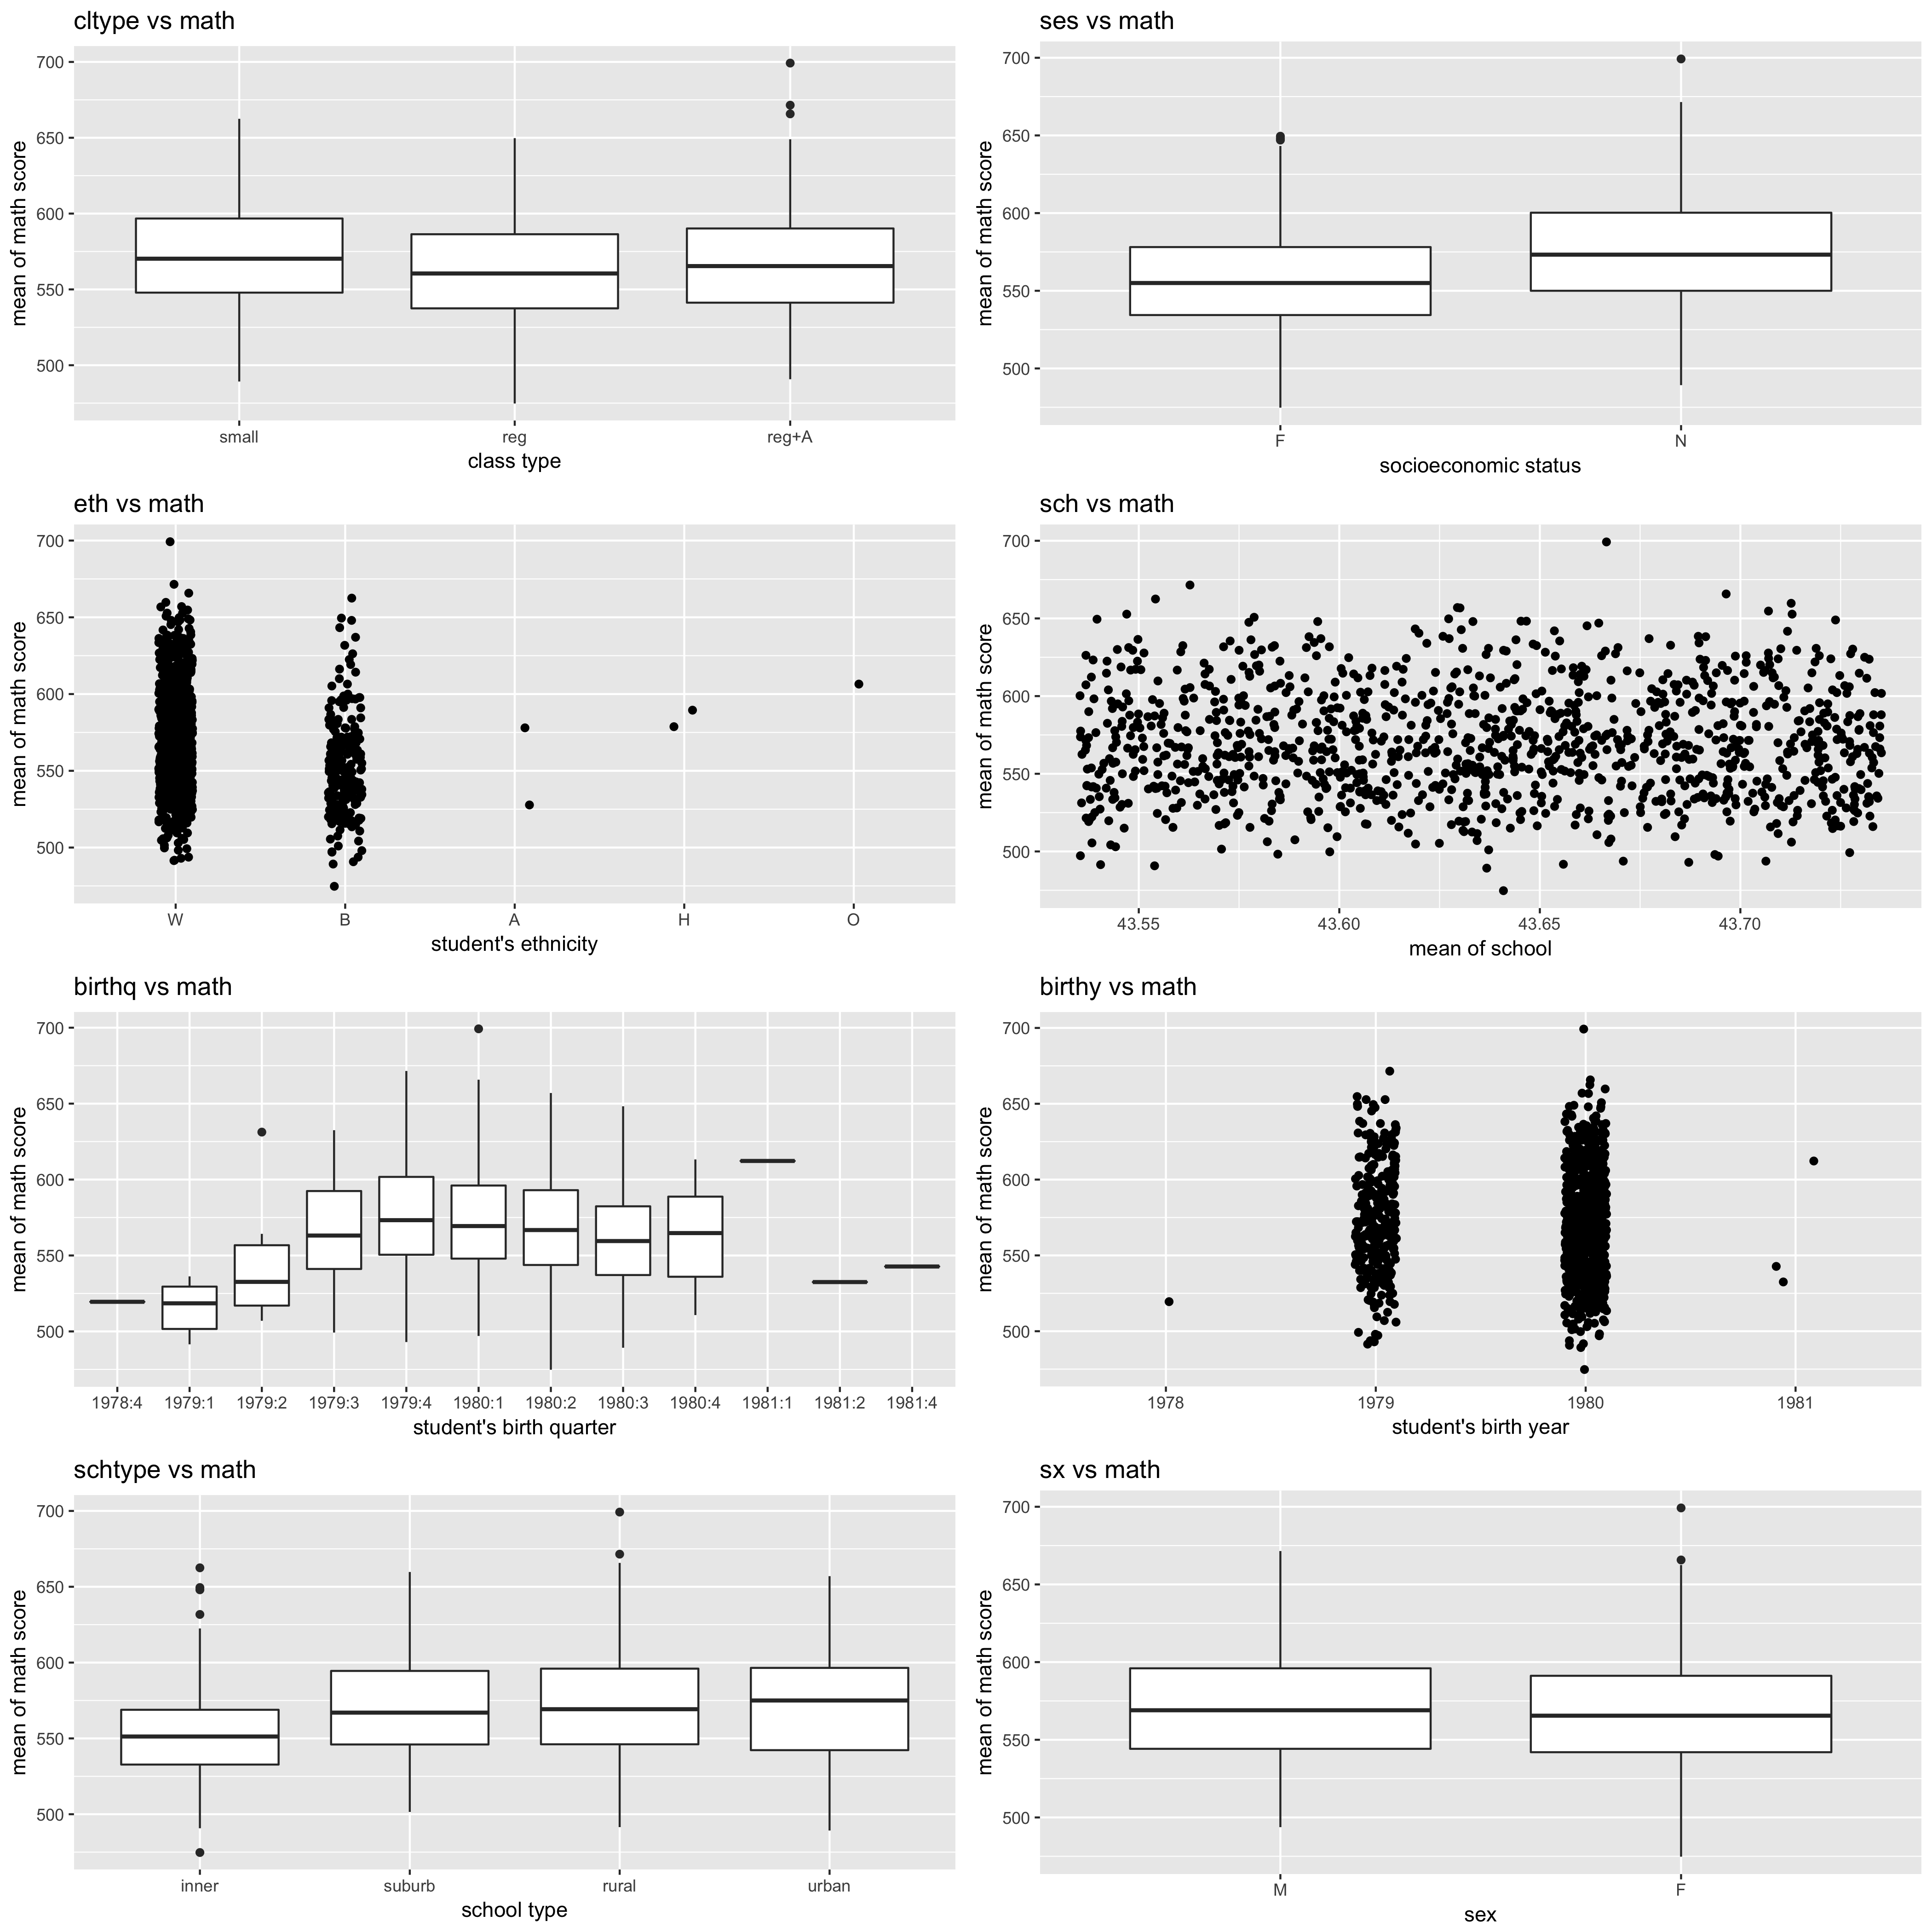
\includegraphics[scale=0.08]{../plot/p24.png}
      }
    \captionof{figure}{Effect of Each Variable}\label{fig:variable}
\end{minipage}\\

Variables like 'ses', 'eth', 'schtype' obviously affect the mean of math score while 'sex' and 'birthy' doesn’t affect much. 
Situation of birthq is more complicated. If quarterly has an effect on score, its influence should be periodic. 
However, the plot between 'birthq' and 'math' shows that this effect seem to be random. So we don't include 'birthq' at the beginning.
Other variables should be examined by model using F-test which can hardly be judged by eyes.

\section{Modeling}

The fixed effects model is inappropriate for this task because it does not take into account the fact that the students are grouped 
by schools. It leads to a violation of the independence of errors assumption. In linear mixed models, we take this by-school 
variability into account by adding adjustment terms u0j which adjust β0 for school j. In our analysis a series of random intercept 
mixed effects models are fitted, with school as random effect and other predictor variables as fixed effects. 

\subsection{Model 0}



First, we build a basic model. Only variable 'sch' is considered as a random effect and all other variables including 'ses', 'eth', 
'cltype', 'se', 'schtype' as fixed effects. The basic model is in this form:

\begin{align*}
    math_i 
    &= \beta_0 + \beta_1*cltype_i + \beta_2*ses_i + \beta_3*eth_i + \beta_4*se_i + \beta_5*schtype_i \\
    &+ sch_{j[i]} + \sigma_e\\
    sch_j &\sim N(0, \sigma_{sch})\\
\end{align*}

\subsection{Model 1}

Since the basic model contains all possible important variables, the next step is to drop the variables that are not significant. 
Backward elimination method here is used to delete variables one by one and the criterion for deleting variables is the F-test. 
Through 'step' function in 'lmerTest' R-package, three variables 'cltype', 'se', 'schtype' are considered as insignigicant, 
and the new model looks like:

\begin{align*}
    math_i &= \beta_0 + \beta_1*cltype_i + \beta_2*ses_i + \beta_3*eth_i + sch_{j[i]} + \sigma_e\\
    sch_j &\sim N(0, \sigma_{sch})\\
\end{align*}

\subsection{Model 2}



\begin{minipage}{\linewidth}
    \makebox[\linewidth]{
      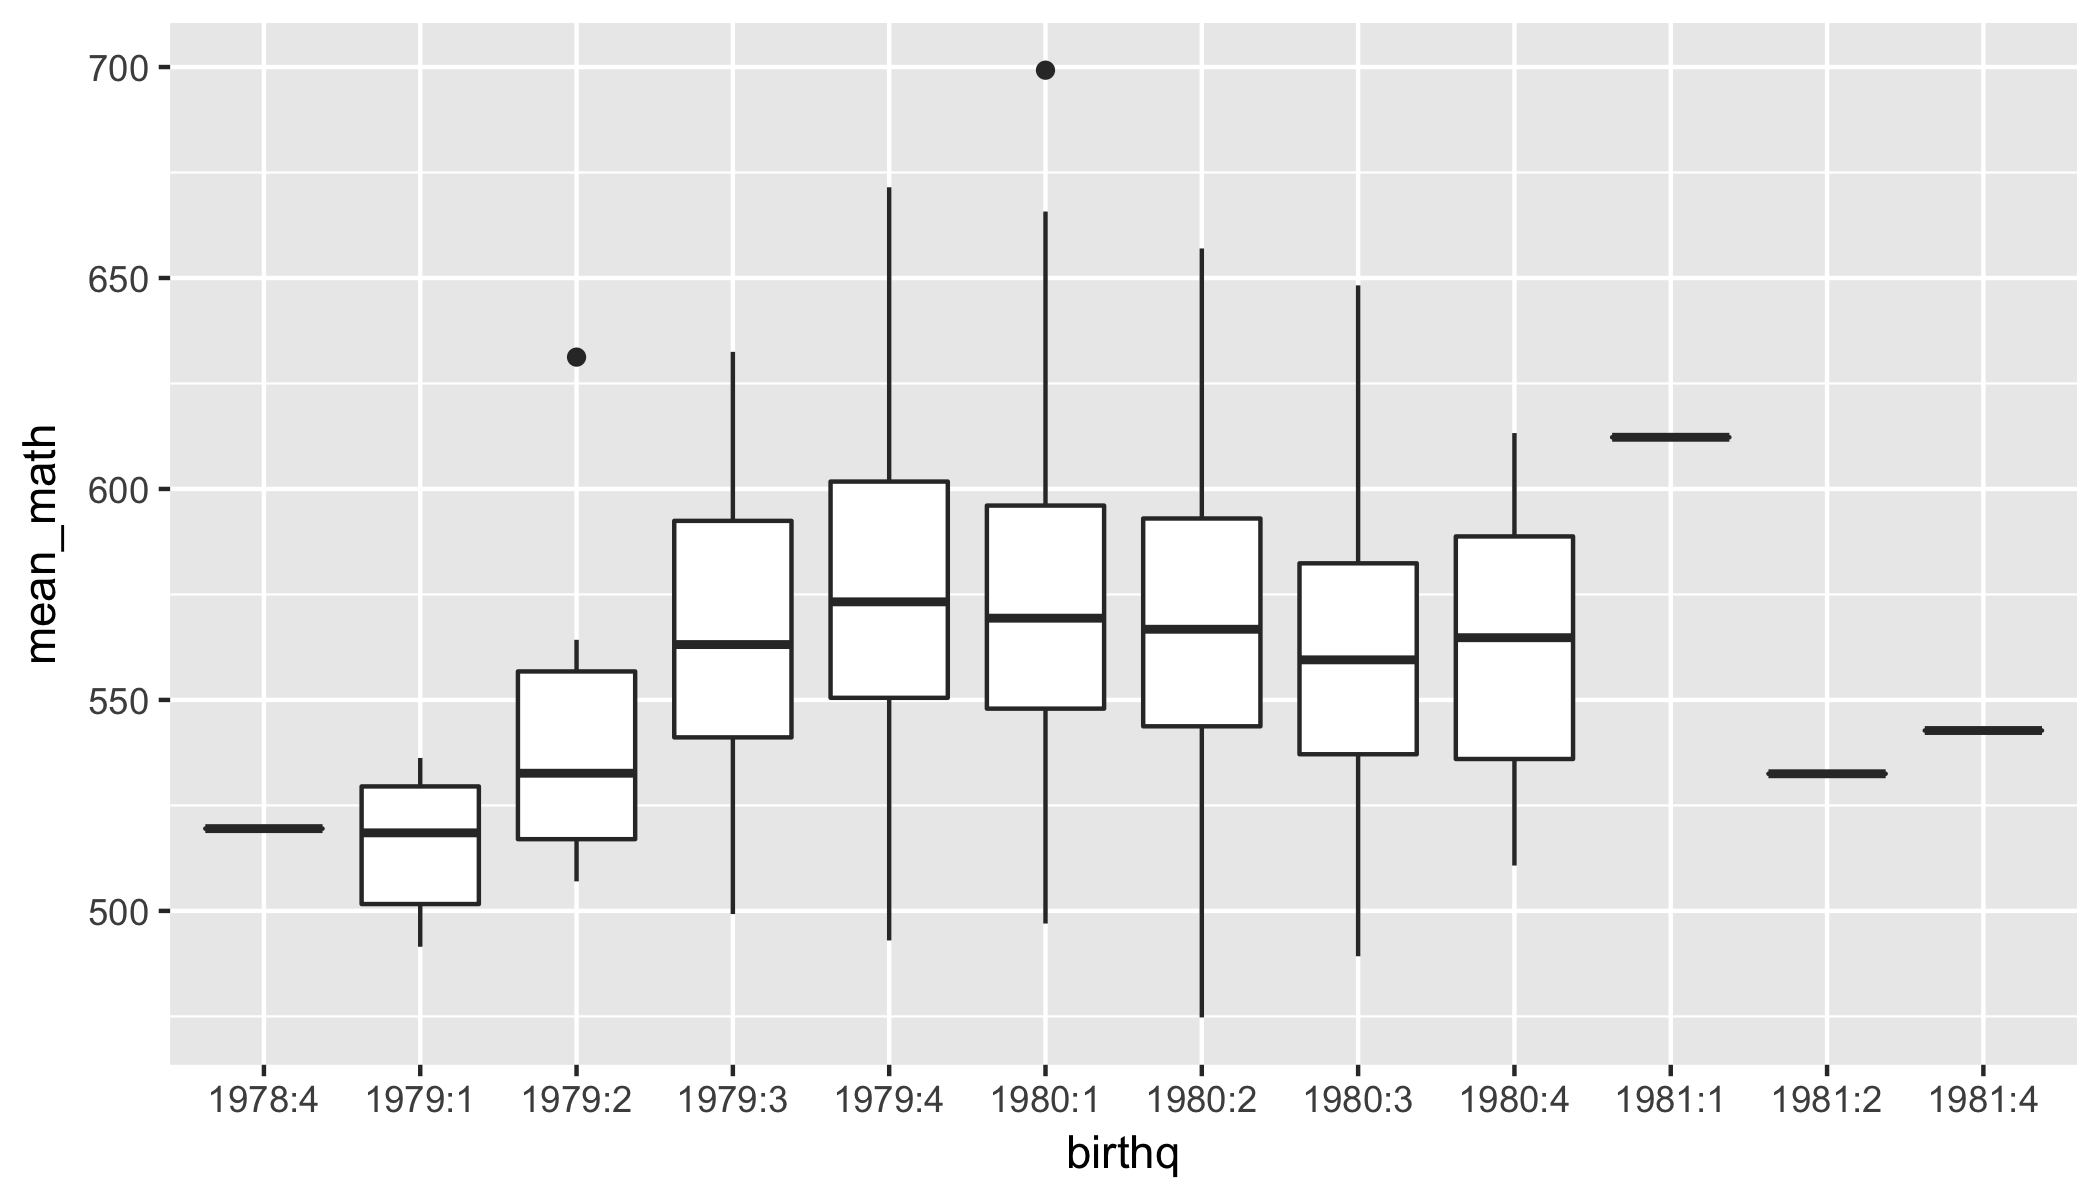
\includegraphics[scale=0.15]{../plot/birthq.png}
      }
    \captionof{figure}{birthq vs math}\label{fig:birthq}
\end{minipage}\\

Form Figure \ref{fig:birthq}, we find that variable 'birthq' has effect on the math score. 
However, if 'birthq' is a fixed effect, its impact on the math score should be cyclical. 
There is no reason to believe that children born in the first quarter are smarter than children born in the second quarter of 1980, 
while the situation in 1979 was the opposite. 
Because of this, variable 'birthq' is added in the model as a random effect. And our model becomes:

\begin{align*}
    math_i &= \beta_0 + \beta_1*cltype_i + \beta_2*ses_i + \beta_3*eth_i + sch_{j[i]} + birthq_{k[i]} + \sigma_e\\
    sch_j &\sim N(0, \sigma_{sch})\\
    birthq_k &\sim N(0, \sigma_{birthq})\\
\end{align*}

\subsection{Model 3}

\begin{minipage}{\linewidth}
    \makebox[\linewidth]{
      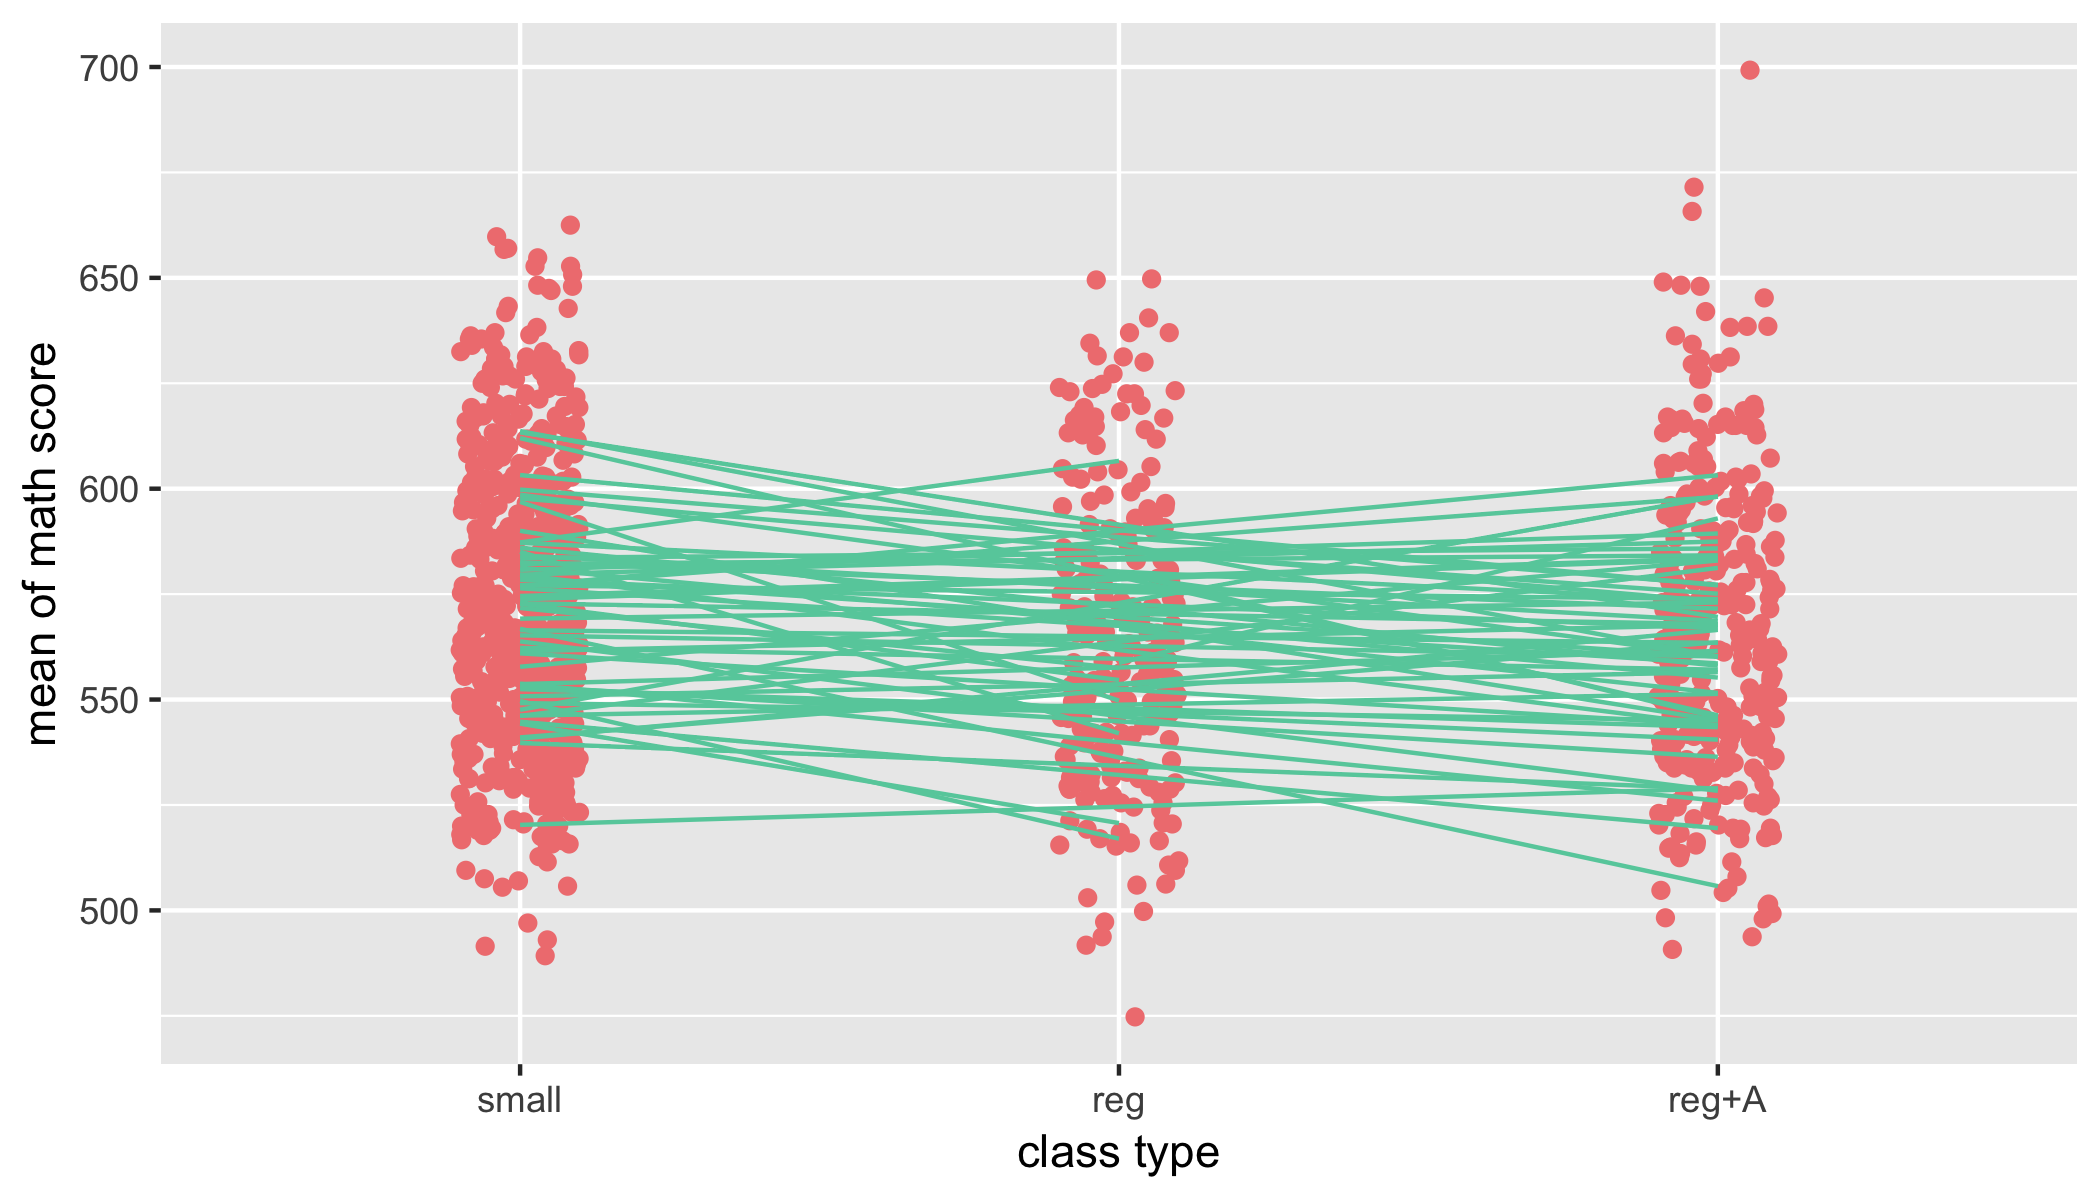
\includegraphics[scale=0.15]{../plot/random_slope.jpg}
      }
    \captionof{figure}{The influence of schools on the relationship between cltype and math}\label{fig:random slope}
\end{minipage}\\

From the plot we can see that the slopes of straight lines vary among different schools. Class type affect the mean of math score, 
but the degrees of the effect are different among schools. Thus, take school as random slope may be a good choice. The model shows below:

\begin{align*}
    math_i &= \beta_{0i} + \beta_{1i}*cltype_i + \beta_2*ses_i + \beta_3*eth_i + \sigma_e\\
    \beta_{0i} &\sim N(sch_{j[i]}, \sigma_1)\\
    \beta_{1i} &\sim N(sch_{j[i]}, \sigma_2)\\
\end{align*}

\subsection{Model Selection}

After building all four models with stan, we find that all estimations all converge. So we use BIC method to select the final model. 
The result is Model $2<3<<1<0$, and since Model 2 is simpler than Model 3, we choose Model 2 as our final model.

\begin{minipage}{\linewidth}
    \makebox[\linewidth]{
      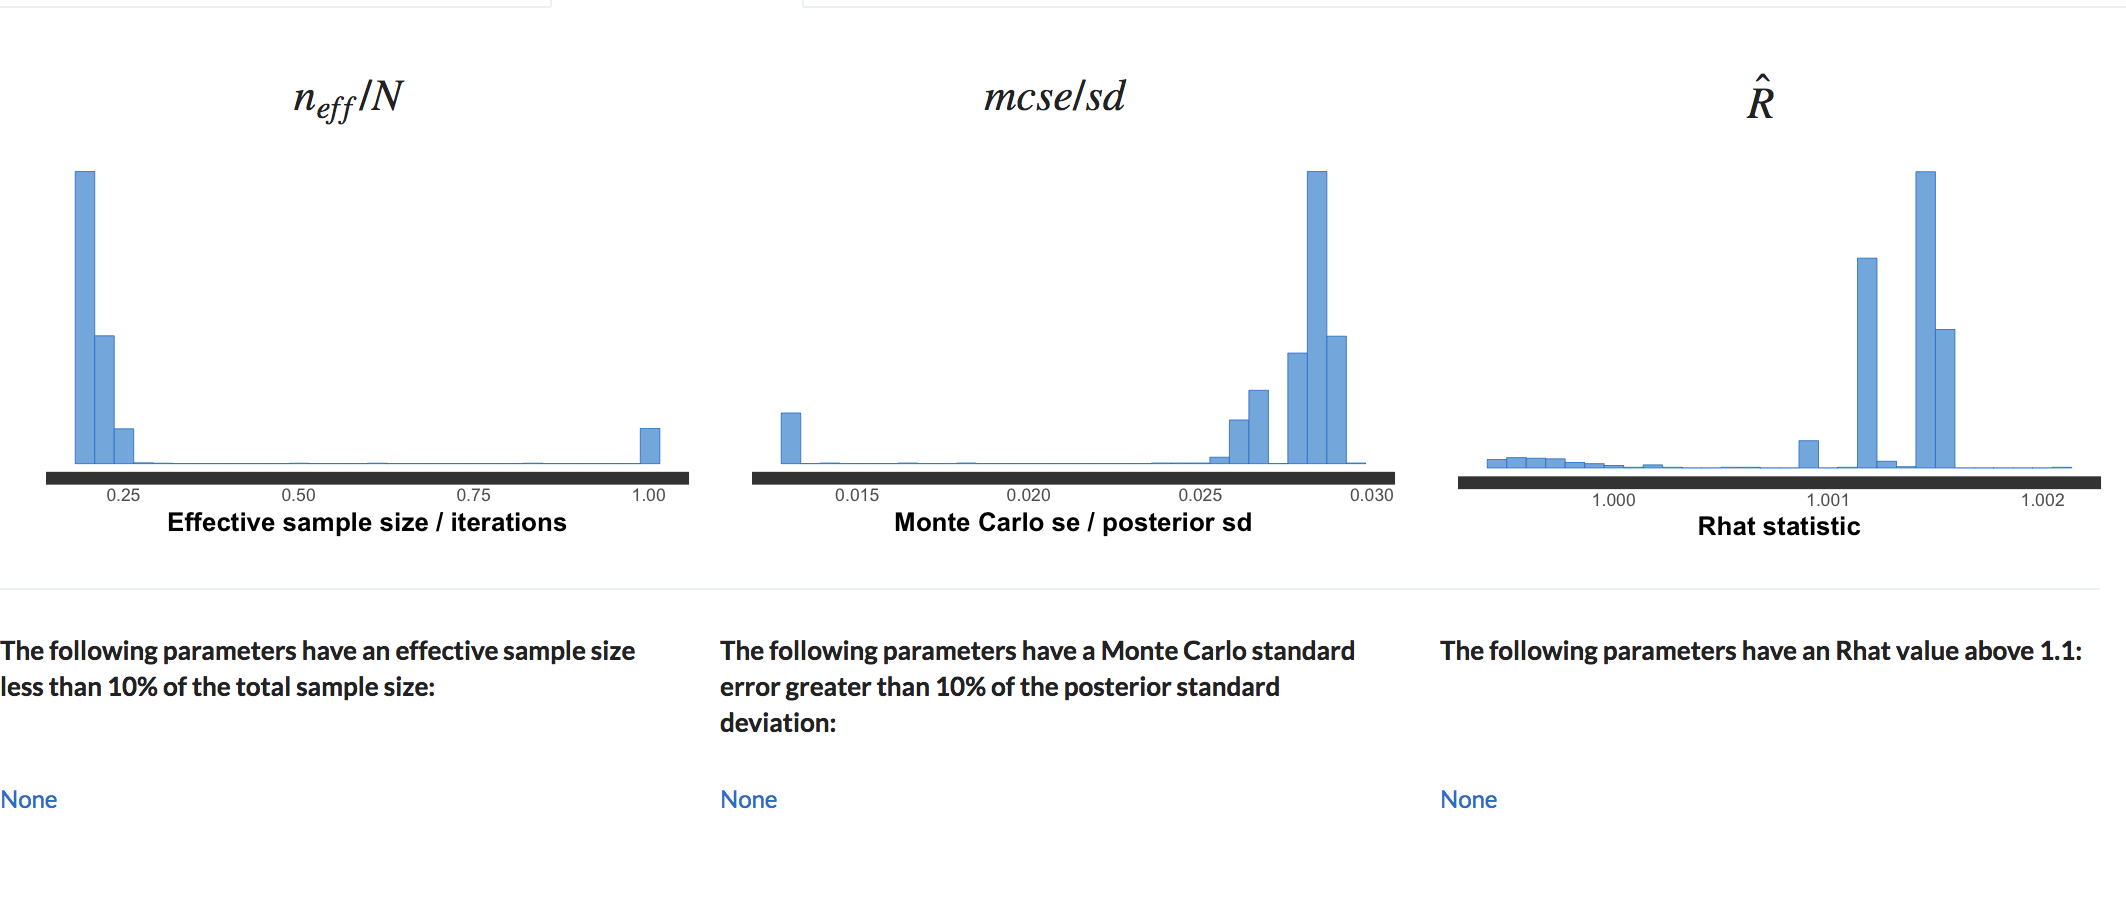
\includegraphics[scale=0.3]{../plot/rhat.jpg}
      }
    \captionof{figure}{Diagnostic of Model 2}\label{fig:rhat}
\end{minipage}\\

From Figure \ref{fig:rhat}, $\hat{R}$ shows that our model converges. Estimations of parameters in model 3 are listed below in 
Table \ref{tab:estimation}. Since the number of levels of the random effect 'sch' exceeds 60, 
only the first two schools' estimates are listed in the table.

\begin{table}[h]
    \centering
    \caption{Estimations of parameters}
    \label{tab:estimation}
    \begin{tabular}{|l|l|l|l|l|l|l|l|l|l|l|}
    \hline
    Variable      & n\_reff & Rhat & mean           & mcse & sd   & 2.5\% & 25\%  & 50\%  & 75\%  & 97.5\% \\ \hline
    Intercept     & 1249    & 1    & 560.2          & 0.2  & 6.3  & 546.9 & 556.4 & 560.4 & 564.1 & 572.1  \\ \hline
    cltype: reg   & 6000    & 1    & \textit{-10.1} & 0    & 2.5  & -15.1 & -11.8 & -10.1 & -8.4  & -5.2   \\ \hline
    cltype: reg+A & 6000    & 1    & \textbf{-9.2}  & 0    & 2.2  & -13.6 & -10.7 & -9.2  & -7.6  & -4.9   \\ \hline
    ses: N        & 6000    & 1    & 14.7           & 0    & 2.3  & 10.1  & 13.2  & 14.7  & 16.2  & 19.2   \\ \hline
    eth: B        & 5061    & 1    & -16.3          & 0    & 3.2  & -22.8 & -18.5 & -16.3 & -14.2 & -10    \\ \hline
    eth: A        & 6000    & 1    & -13.4          & 0.3  & 22.4 & -57.5 & -28.7 & -13.2 & 1.8   & 30.4   \\ \hline
    eth: H        & 6000    & 1    & 4.4            & 0.3  & 21.7 & -37.6 & -10.7 & 4.6   & 19.1  & 46     \\ \hline
    eth: O        & 6000    & 1    & 18.3           & 0.4  & 30.7 & -42   & -2    & 18.4  & 38.9  & 77.6   \\ \hline
    sch: 2        & 6000    & 1    & 6.3            & 0.1  & 7.1  & -7.4  & 1.5   & 6.2   & 11    & 20.6   \\ \hline
    sch: 3        & 6000    & 1    & -12.2          & 0.1  & 9.1  & -30.6 & -18.5 & -12.1 & -5.9  & 5      \\ \hline
    \end{tabular}
\end{table}

The estimate of 'cltype: reg' is $-10.1$ which is negative. It shows that students in small class type significantly have better 
performance in math than those in regular class. The estimate of 'cltype: reg+A' is $-9.2$, slightly larger than $-10.1$. 
And this tells us that teachers aide slightly improve students’ math performance, but small class type is still much better than it.\\

The estimate of 'ses: N' is $14.7$ and this positive estimation means that students who are not eligible for free lunches have
better performance. This is in line with our intuition because those students usually come from wealthy families and their 
parents can provide them with better learning resources.\\

The estimate of different 'eth' indicates that students with different trace tend to have different performance.\\

\section{Summary}

The final model answers research question: 
\begin{itemize}
    \item class size significantly affects performance of students on math.
    \item 'ses' along with 'eth' also have influence on performance of students on math.
\end{itemize}

We also compare our model with regular linear model $math ~ cltype + ses + eth$.

\begin{table}[h]
    \centering
    \caption{Comparison between linear model and multilevel model}
    \label{tab:lm}
    \begin{tabular}{|l|l|l|l|l|l|l|l|l|}
    \hline
    Model            & Intercept & reg         & reg+A         & ses: N & eth: B & eth: A & eth:  H & eth: O \\ \hline
    Linear Model     & 576.9     & -9.5        & -8,9          & 16.4   & -20.5  & -5.6   & 4.9     & 22.5   \\ \hline
    Multilevel Model & 560.2     & -10.1       & -9.2          & 14.7   & -16.3  & -13.4  & 4.4     & 18.3   \\ \hline
    \end{tabular}
\end{table}

From Table \ref{tab:lm}, we can see that the estimates of coefficients in both models are slightly different except 
'eth: B' and 'eth: A'. After calculating BIC, Multilevel Model is better than Linear Model.

\section{Future Work}

All our analysis above focus on factors affect math scores, if given more time we can take a look at the factors which affect the 
read scores. It’s interesting to see whether two sets of factors are the same or not.\\

If time permits, more interesting questions can be discussed. Based on the whole dataset, we are curious to find if class type 
affect the test scores when the grade goes up. Or what differences will be made on the test scores if a student change the class 
type even change the school during the four consecutive years. We can both discuss the student level and school level which are 
more complex.\\

What’s more, there are six levels of student’s ethnicity in the full dataset while five levels in the subset. The change of 
effect of ethnicity on test scores is worth to discuss.


\end{document}